Searching for particle Dark Matter can be done using three mechanisms: indirect detection by searching for signals from annihilation products; production at particle colliders and direct detection via scattering off target nuclei. Figure \ref{fig:detection_schem} illustrates the possible Dark Matter detection methods and how an ordinary matter particle, P, would couple to a potential Dark Matter candidate, $\chi$.
\begin{figure}[h]
    \centering
    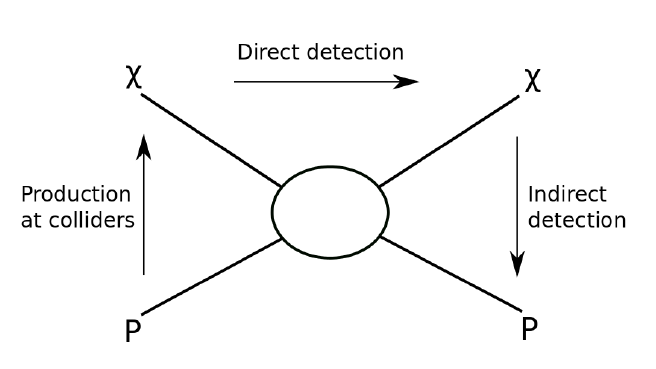
\includegraphics[width=0.7\textwidth]{Figures/Detection_schematic.png}
    \caption{Schematic illustrating the three possible Dark Matter detection methods: production of Dark Matter particles from the collision of ordinary matter (upwards); detection of recoil products (left to right); and dark matter particles annihilating to produce ordinary matter (downwards) \cite{DirectDetection2015}}
    \label{fig:detection_schem}
\end{figure}
\section{Indirect detection of Dark Matter}\label{sec:indirect}
An increase in Dark Matter density form halos around astronomical objects such as stars and galaxies which make these sources ideal regions in which to conduct indirect Dark Matter searches. The Dark Matter flux produced in these regions of higher density could be used to measure its presence due to scattering, self annihilation and decays into standard model particles. By detecting these decay products, it could infer the existence of Dark Matter. The possible decay channels can be seen in equations \ref{eqn:DMGAMMA} and \ref{eqn:DMBARY} \cite{DMProd}:
\begin{equation}\label{eqn:DMGAMMA}
    \chi\Bar{\chi} \rightarrow \gamma\gamma,\: \gamma Z,\: \gamma H \quad \textrm{or}
\end{equation}
\begin{equation}\label{eqn:DMBARY}
    \chi\Bar{\chi} \leftrightarrow e^+e^-,\: \mu^+\mu^-,\: q\Bar{q},\: W^+W^-,\: ZZ,\: HH\: ...
\end{equation}
There are many other possible indirect detection mechanisms that can be searched for such as observing high energy $\gamma-\textrm{rays}$ using atmospheric Cherenkov telescopes pointed in the direction of objects with expected high levels of Dark Matter or detecting neutrinos which radiate out of the sun after capture \cite{DirectDetection2015}. 

\section{Dark Matter production at colliders}\label{sec:colliders}
The production of Dark Matter at particle colliders is a well motivated method in which observing events with missing transverse momentum and energy would infer the possible presence of a WIMP. Since 2008, the ATLAS and CMS experiments on the Large Hadron Collider at CERN have used proton-proton collisions with a centre of mass energy of $7\:TeV\textrm{ to }13\:TeV$ to search for new particles. The mechanism in which a particle collider would detect a WIMP-like can be seen in equation \ref{eqn:DMCOLLIDER} where $p$ represents proton and $x$ could be either a hadronic jet, a photon or leptonically decaying Z or W boson \cite{DirectDetection2015}.
\begin{equation}\label{eqn:DMCOLLIDER}
   pp \rightarrow \chi\Bar{\chi} + x
\end{equation}
Results remain consistent with standard model expectations from analysis of the data from collision events. With the forthcoming upgrade of the LHC, increased luminosity's and collision energies will allow for a larger parameter space to be analysed.

\section{Direct detection of Dark Matter}\label{sec:directdetection}
The direct detection of Dark Matter involves the identification of nuclear recoils produced from the collision of Dark Matter particle, a WIMP, with a detector's target nuclei. The nuclear recoils observed would be in the range of $1-100\:keV$ from a collision of WIMP with a mass of $10-1000\:GeV/c^2$ \cite{DirectDetection2015}. The signal produced by the nuclear recoil can be observed by one of three different forms: phonons or heat; charge; and light. A detector will be designed with the corresponding technologies to detect one or two of the possible three signals. A schematic of this process can be seen in figure \ref{fig:Direct}.
\begin{figure}[h]
    \centering
    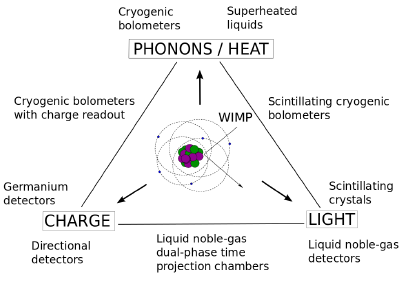
\includegraphics[width=0.7\textwidth]{Figures/Direct_direction.png}
    \caption{A schematic showing the possible direct detection signals and the corresponding experiments used to observe such signals.\cite{DirectDetection2015}}
    \label{fig:Direct}
\end{figure}
The LUX-ZEPLIN (LZ) experiment will observe signals of both light and charge by utilising a liquid Xenon dual phase time projection chamber, this method will be described in chapter \ref{Chap5:LZ}.
\newline
The three different detection techniques discussed in this chapter collectively cover the range set on the parameter space in which the WIMP cross-section lies. If one of the methods were to be successful in identifying a WIMP, the result would then be verified with one or combination of the two remaining methods.